% Πρόβλεψη κίνησης κινητού δικτύου
% Build: xelatex slides.tex (run twice), or: tectonic slides.tex
% Data for the charts: python presentation/export_data.py (raw data, from the repo root)
%                      %run -i presentation/slide_figures.py (forecasts, last cell of the notebook)
% Speaker notes: uncomment the \setbeameroption line below to get slides + notes side by side.
\documentclass[aspectratio=169,10pt]{beamer}

\usetheme{metropolis}
\metroset{sectionpage=none, progressbar=frametitle, numbering=fraction, block=fill}
\usefonttheme{professionalfonts}
% \setbeameroption{show notes on second screen=right}

% ---------- fonts and language ----------
\usepackage{fontspec}
\usepackage{polyglossia}
\setmainlanguage{greek}
\setotherlanguage{english}
\setmainfont{FiraSans}[
  Extension = .otf, UprightFont = *-Book, BoldFont = *-SemiBold,
  ItalicFont = *-BookItalic, BoldItalicFont = *-SemiBoldItalic]
\setsansfont{FiraSans}[
  Extension = .otf, UprightFont = *-Book, BoldFont = *-SemiBold,
  ItalicFont = *-BookItalic, BoldItalicFont = *-SemiBoldItalic]
\setmonofont{FiraMono}[Extension = .otf, UprightFont = *-Regular, BoldFont = *-Medium, Scale = 0.92]
\usepackage{unicode-math}
\setmathfont{FiraMath-Regular.otf}

\usepackage{booktabs}
\usepackage{array}
\usepackage{graphicx}
\usepackage{algpseudocode}
\usepackage{tikz}
\usetikzlibrary{positioning, arrows.meta}
\usepackage{pgfplots}
\usepgfplotslibrary{groupplots}
\pgfplotsset{compat=1.18}
\graphicspath{{figs/}}

% ---------- colours ----------
% Rule: colour only ever means a series (same colours as the notebook figures).
% Everything else is neutral: models are told apart by line style and shade, emphasis is weight.
% Flat fills, no borders, no rounded corners.
\definecolor{inet}{HTML}{2A78D6}
\definecolor{sms}{HTML}{EB6834}
\definecolor{calls}{HTML}{1BAF7A}
\definecolor{ink}{HTML}{16202A}
\definecolor{text}{HTML}{2B3640}
\definecolor{paper}{HTML}{F7F8FA}
\definecolor{fillc}{HTML}{E8ECF0}
\definecolor{rule}{HTML}{D5DBE1}
\definecolor{muted}{HTML}{66727F}
\definecolor{quiet}{HTML}{8A96A3}

% Stock metropolis look. One override: alerts are bold dark grey instead of orange,
% because orange already means the SMS series in every chart.
\setbeamercolor{alerted text}{fg=mDarkTeal}
\setbeamerfont{alerted text}{series=\bfseries}
\algrenewcommand{\algorithmiccomment}[1]{\hfill{\footnotesize\textcolor{muted}{// #1}}}

\newcommand{\muted}[1]{\textcolor{muted}{#1}}
\newcommand{\figcap}[1]{\par\vspace{2pt}{\scriptsize\muted{#1}}}
% series names with their colour key, as in the figures
\newcommand{\ser}[2]{\textcolor{#1}{\rule[0.05em]{0.6em}{0.6em}}\,#2}
\newcommand{\sInet}{\ser{inet}{Internet}}
\newcommand{\sSms}{\ser{sms}{SMS}}
\newcommand{\sCalls}{\ser{calls}{Calls}}

% ---------- chart style ----------
\pgfplotsset{deck/.style={
  axis x line*=bottom, axis y line*=left, axis line style={draw=rule}, tick style={draw=rule},
  tick label style={font=\tiny, text=muted}, label style={font=\scriptsize, text=muted},
  /pgf/number format/.cd, 1000 sep={.}, use comma, /pgfplots/.cd,
  legend style={draw=none, fill=none, font=\scriptsize, text=text},
  title style={font=\scriptsize, text=ink, anchor=south west, at={(0,1)}, yshift=-1pt}}}

% ---------- title ----------
\title{Πρόβλεψη κίνησης κινητού δικτύου}
\subtitle{Ένα τετράγωνο του Μιλάνου, δύο μήνες δεδομένων, τρεις οικογένειες μοντέλων}
\author{Παναγιώτης Πολυμέρος, Βασίλης Μυλωνάς}
\institute{Αρχιτεκτονικές Δικτύων Επόμενης Γενιάς, επιβλέπων Γιάννης Λακουμέντας}
\date{}

\begin{document}

% =====================================================================
\maketitle
\note{Καλησπέρα. Θα παρουσιάσουμε την πρόβλεψη κίνησης για ένα τετράγωνο του Μιλάνου, το 5060. Θέλουμε να προβλέψουμε την κίνηση δέκα έως πενήντα λεπτά μπροστά.}

% =====================================================================
\begin{frame}{Ίδια διαδικασία για κάθε μοντέλο}
  \vspace{0.6em}
  \centering
  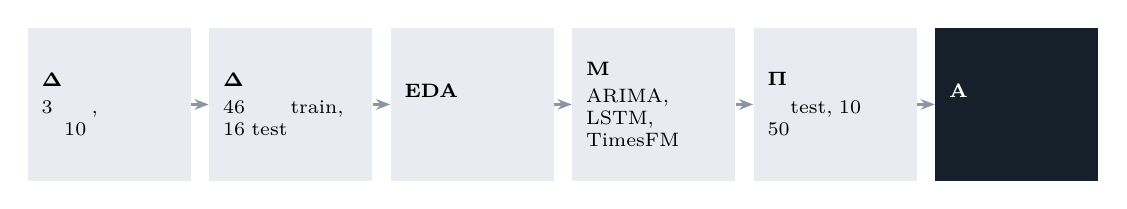
\begin{tikzpicture}[node distance=0.22cm, >={Stealth[length=1.8mm]},
      stage/.style={fill=fillc, text width=1.72cm, minimum height=1.95cm, align=left,
                   inner xsep=5pt, inner ysep=5pt, font=\scriptsize},
      key/.style={fill=ink, text=white, text width=1.72cm, minimum height=1.95cm, align=left,
                  inner xsep=5pt, inner ysep=5pt, font=\scriptsize}]
    \node[stage] (a) {\textbf{Δεδομένα}\\[2pt] 3 σειρές, ένα σημείο ανά 10 λεπτά};
    \node[stage, right=of a] (b) {\textbf{Διαχωρισμός}\\[2pt] 46 ημέρες train, 16 test};
    \node[stage, right=of b] (c) {\textbf{EDA}\\[2pt] κύκλοι και γιορτές};
    \node[stage, right=of c] (d) {\textbf{Μοντέλα}\\[2pt] ARIMA, LSTM, TimesFM};
    \node[stage, right=of d] (e) {\textbf{Πρόβλεψη}\\[2pt] στο test, 10 και 50 λεπτά μπροστά};
    \node[key,  right=of e] (f) {\textbf{Αποτίμηση}\\[2pt] έναντι απλών κανόνων};
    \foreach \u/\v in {a/b, b/c, c/d, d/e, e/f} \draw[->, thick, quiet] (\u) -- (\v);
  \end{tikzpicture}

  \vspace{1.4em}
  \raggedright
  \begin{itemize}
    \item Κάθε επιλογή (παράμετροι, αρχιτεκτονική, ποιο μοντέλο εκπροσωπεί κάθε οικογένεια) γίνεται \alert{μόνο στο train}.
    \item Όλα τα μοντέλα προβλέπουν από τα \alert{ίδια σημεία} του test, για τους ίδιους ορίζοντες.
    \item Ένα μοντέλο αξίζει μόνο αν νικά τον απλό κανόνα «η κίνηση θα μείνει όπως είναι».
  \end{itemize}
\end{frame}
\note{Αυτή είναι η διαδικασία από την αρχή ως το τέλος, και η παρουσίαση την ακολουθεί με την ίδια σειρά. Το σημαντικό είναι ότι όλες οι αποφάσεις γίνονται στο train και ότι όλα τα μοντέλα αξιολογούνται με τον ίδιο τρόπο, ώστε η σύγκριση στο τέλος να είναι δίκαιη.}

% =====================================================================
\begin{frame}{Με πρόβλεψη, το δίκτυο δρα πριν τη συμφόρηση}
  Στα 5G/6G πολλές λειτουργίες είναι λογισμικό, οπότε οι πόροι αλλάζουν δυναμικά.

  \vspace{1em}
  \centering
  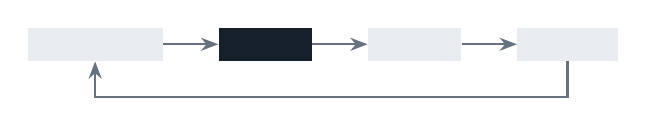
\begin{tikzpicture}[node distance=0.7cm, >={Stealth[length=2.2mm]},
      box/.style={fill=fillc, inner xsep=8pt, inner ysep=6pt, font=\small}]
    \node[box] (m) {παρακολούθηση};
    \node[box, right=of m, fill=ink, text=white, font=\small\bfseries] (a) {ανάλυση};
    \node[box, right=of a] (d) {απόφαση};
    \node[box, right=of d] (e) {εκτέλεση};
    \draw[->, thick, muted] (m) -- (a);
    \draw[->, thick, muted] (a) -- (d);
    \draw[->, thick, muted] (d) -- (e);
    \draw[->, thick, muted] (e.south) -- ++(0,-0.45) -| (m.south);
  \end{tikzpicture}
  \figcap{Ο κλειστός βρόχος του ZSM (ETSI). Η πρόβλεψη είναι το βήμα της ανάλυσης.}

  \vspace{1.2em}
  \raggedright
  \begin{columns}[T, onlytextwidth]
    \begin{column}{0.48\textwidth}
      \muted{Short-term}\\[2pt]
      {\large\textbf{το επόμενο δεκάλεπτο}}
    \end{column}
    \begin{column}{0.48\textwidth}
      \muted{Long-term}\\[2pt]
      {\large\textbf{τα επόμενα 50 λεπτά}}
    \end{column}
  \end{columns}
  \vspace{0.8em}
  \muted{Αρκετός χρόνος για να ξυπνήσει μια κυψέλη ή να κλιμακωθεί μια εικονική λειτουργία.}
\end{frame}
\note{Το ZSM του ETSI ορίζει έναν κλειστό βρόχο: παρακολούθηση, ανάλυση, απόφαση, εκτέλεση. Η πρόβλεψη κίνησης είναι το στάδιο της ανάλυσης· χωρίς αυτήν ο βρόχος αντιδρά αφού έχει ήδη έρθει η συμφόρηση. Σε κάθε στιγμή κάνουμε δύο προβλέψεις: το επόμενο δεκάλεπτο και τα πέντε επόμενα. Αντίστροφα, όταν προβλέπεται χαμηλό φορτίο, μπορούμε να κλείσουμε εξοπλισμό, αλλά μόνο αν εμπιστευόμαστε την πρόβλεψη.}

% =====================================================================
\begin{frame}{Ένα τετράγωνο στο Duomo, τρεις σειρές}
  \begin{columns}[T, onlytextwidth]
    \begin{column}{0.48\textwidth}
      \begin{itemize}
        \item Telecom Italia, \emph{Big Data Challenge 2014}: Call Detail Records, 01/11/2013 έως 01/01/2014.
        \item Ένα σημείο ανά δεκάλεπτο: \alert{8.928 σημεία} ανά σειρά, χωρίς κενά.
        \item Οι τιμές είναι κλιμακωμένες με κρυφή σταθερά: \alert{δεν έχουν μονάδα}.
      \end{itemize}
    \end{column}
    \begin{column}{0.48\textwidth}
      \small
      \begin{tabular}{@{}ll@{}}
        \toprule
        Σειρά & Ποιον πόρο φορτώνει \\
        \midrule
        \sInet & User plane: ραδιοπόροι, UPF \\
        \sSms & Σηματοδοσία (AMF, SMSF) \\
        \sCalls & Φωνή με εγγυημένο ρυθμό \\
        \bottomrule
      \end{tabular}
    \end{column}
  \end{columns}
  \vspace{1em}
  \begin{block}{Τι πρέπει να έχουμε υπόψη}
    Το Internet μετρά εγγραφές, όχι bytes. Βλέπουμε μόνο έναν πάροχο, έως το 34\% του πληθυσμού. Τα δεδομένα είναι του 2013, πριν το 5G.
  \end{block}
  \figcap{Πηγή: Barlacchi et al., \emph{Scientific Data}, 2015.}
\end{frame}
\note{Κρατήσαμε μόνο το τετράγωνο 5060, πάνω στην Piazza del Duomo, περίπου 235 επί 235 μέτρα. Αθροίζουμε εισερχόμενα και εξερχόμενα, και όλους τους κωδικούς χώρας, γιατί εξυπηρετούνται από τους ίδιους σταθμούς βάσης. Οι τιμές είναι κλιμακωμένες με μια κρυφή σταθερά, άρα ένα σφάλμα 50 δεν σημαίνει 50 Mbps ή 50 κλήσεις: τα σφάλματα τα διαβάζουμε σχετικά.}

% =====================================================================
\begin{frame}{Μαθαίνουμε στο φθινόπωρο, ελέγχουμε στις γιορτές}
  \centering
  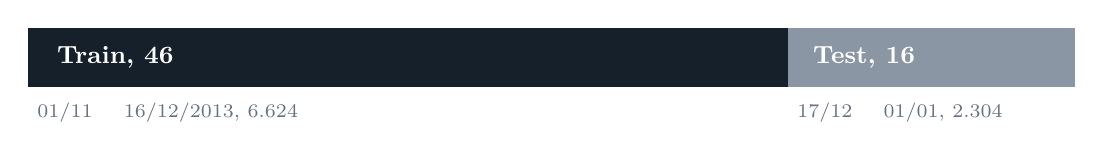
\begin{tikzpicture}
    \fill[ink]   (0,0) rectangle (9.65,0.75);
    \fill[quiet] (9.65,0) rectangle (13.3,0.75);
    \node[anchor=west, text=white, font=\small\bfseries] at (0.25,0.375) {Train, 46 ημέρες};
    \node[anchor=west, text=white, font=\small\bfseries] at (9.85,0.375) {Test, 16 ημέρες};
    \node[anchor=north west, text=muted, font=\scriptsize] at (0,-0.08) {01/11 έως 16/12/2013, 6.624 σημεία};
    \node[anchor=north west, text=muted, font=\scriptsize] at (9.65,-0.08) {17/12 έως 01/01, 2.304 σημεία};
  \end{tikzpicture}

  \vspace{1.6em}
  \raggedright
  \begin{itemize}
    \item Χωρίζουμε \alert{στον χρόνο}: ένας τυχαίος διαχωρισμός θα έδινε στο μοντέλο τιμές από το μέλλον.
    \item Το test είναι το τελευταίο τέταρτο, σε ολόκληρες ημέρες.
    \item Πέφτει πάνω σε Χριστούγεννα και Πρωτοχρονιά, που το train δεν έχει δει ποτέ. Αυτό θα αλλάξει ποιο μοντέλο κερδίζει.
  \end{itemize}
\end{frame}
\note{Η εκφώνηση προτείνει 1/3 ή 1/4· κρατάμε το τελευταίο τέταρτο, στρογγυλεμένο σε ολόκληρες ημέρες. Το test ελέγχει έτσι και συνθήκες που τα μοντέλα δεν έχουν δει, και θα δούμε ότι αυτό αλλάζει ποιο μοντέλο κερδίζει.}

% =====================================================================
\begin{frame}{Ο ημερήσιος κύκλος κυριαρχεί, οι γιορτές τον σπάνε}
  \begin{columns}[T, onlytextwidth]
    \begin{column}{0.62\textwidth}
      \begin{tikzpicture}
        \begin{groupplot}[deck, group style={group size=1 by 3, vertical sep=0.78cm, xticklabels at=edge bottom},
            width=0.9\linewidth, height=1.15cm, scale only axis, xmin=0, xmax=62, ymin=0,
            xtick={0,9,16,23,30,37,46,53,61}, xticklabels={1/11,10/11,17/11,24/11,1/12,8/12,17/12,24/12,1/1},
            yticklabel style={/pgf/number format/fixed}, ytick distance=500]
          \nextgroupplot[ymax=1700, title={\ser{inet}{Internet}}]
            \addplot[fill=fillc, draw=none, const plot] table[x=x, y expr=\thisrow{off}*1700] {figs/series_hourly.dat} \closedcycle;
            \addplot[inet, line width=0.35pt] table[x=x, y=internet] {figs/series_hourly.dat};
            \draw[ink, dashed] (axis cs:46,0) -- (axis cs:46,1700);
          \nextgroupplot[ymax=1100, title={\ser{sms}{SMS}}]
            \addplot[fill=fillc, draw=none, const plot] table[x=x, y expr=\thisrow{off}*1100] {figs/series_hourly.dat} \closedcycle;
            \addplot[sms, line width=0.35pt] table[x=x, y=sms] {figs/series_hourly.dat};
            \draw[ink, dashed] (axis cs:46,0) -- (axis cs:46,1100);
          \nextgroupplot[ymax=380, ytick distance=150, title={\ser{calls}{Calls}}]
            \addplot[fill=fillc, draw=none, const plot] table[x=x, y expr=\thisrow{off}*380] {figs/series_hourly.dat} \closedcycle;
            \addplot[calls, line width=0.35pt] table[x=x, y=calls] {figs/series_hourly.dat};
            \draw[ink, dashed] (axis cs:46,0) -- (axis cs:46,380);
        \end{groupplot}
      \end{tikzpicture}
      \figcap{Ωριαίος μέσος. Γκρι: Σαββατοκύριακα και αργίες. Διακεκομμένη: αρχή του test.}
    \end{column}
    \begin{column}{0.35\textwidth}
      \small
      \begin{itemize}
        \item Το μεσημέρι το Internet είναι \alert{\textasciitilde 9 φορές} το νυχτερινό.
        \item Το Σαββατοκύριακο SMS και κλήσεις πέφτουν στο 55–69\% μιας εργάσιμης.
        \item Τα Χριστούγεννα η κίνηση πέφτει στο \alert{16–39\%}, την Πρωτοχρονιά εκτινάσσεται.
        \item Καμία τάση. Οι σειρές μοιάζουν μόνο λόγω του κοινού κύκλου: \alert{κάθε σειρά χωριστά}.
      \end{itemize}
    \end{column}
  \end{columns}
\end{frame}
\note{Το πρώτο που φαίνεται είναι ο ημερήσιος κύκλος. Τις καθημερινές η κορυφή είναι γύρω στο μεσημέρι, το Σαββατοκύριακο μετατοπίζεται στο απόγευμα. Τα SMS και οι κλήσεις πέφτουν το Σαββατοκύριακο, ενώ το Internet σχεδόν δεν αλλάζει, και τη νύχτα του Σαββατοκύριακου είναι πάνω από τριπλάσιο. Στο train οι σειρές έχουν συσχέτιση γύρω στο 0,9, αλλά αν αφαιρέσουμε τον κοινό κύκλο πέφτει στο 0,4, οπότε προβλέπουμε κάθε σειρά μόνη της. Δύο συμπεράσματα για τα μοντέλα: ο τύπος ημέρας αξίζει να δοθεί ως είσοδος, και στις γιορτές του test περιμένουμε μεγαλύτερα σφάλματα.}

% =====================================================================
\begin{frame}{Το ARIMA χρειάζεται βοήθεια για τον ημερήσιο κύκλο}
  \begin{columns}[T, onlytextwidth]
    \begin{column}{0.48\textwidth}
      \begin{block}{SARIMA}
        Μοντελοποιεί τη διαφορά από \alert{χθες την ίδια ώρα}, και ένα μικρό ARMA για ό,τι μένει.
        \vspace{0.4em}

        \small\muted{Ακριβό: \textasciitilde 22 λεπτά ανά fit, γιατί κουβαλά μια ολόκληρη ημέρα στη μνήμη του.}
      \end{block}
    \end{column}
    \begin{column}{0.48\textwidth}
      \begin{block}{ARIMA-x}
        Περιγράφει τον κύκλο με \alert{γνωστές μεταβλητές}: ημιτονοειδείς όρους ημέρας και εβδομάδας, και δείκτη αργίας.
        \vspace{0.4em}

        \small\muted{Γρήγορο: \textasciitilde 11 δευτερόλεπτα ανά fit.}
      \end{block}
    \end{column}
  \end{columns}
  \vspace{1em}
  \begin{columns}[c, onlytextwidth]
    \begin{column}{0.48\textwidth}
      \small
      \begin{tabular}{@{}lcc@{}}
        \toprule
        Τάξη (BIC) & SARIMA & ARIMA-x \\
        \midrule
        \sInet & (2,0,1) & (1,0,1) \\
        \sSms & (2,0,1) & (2,0,1) \\
        \sCalls & (6,0,0) & (1,0,1) \\
        \bottomrule
      \end{tabular}
    \end{column}
    \begin{column}{0.48\textwidth}
      Και στα δύο οι τάξεις βγαίνουν \alert{μικρές}: ο κύκλος κάνει τη βαριά δουλειά, και μένει λίγη μνήμη για το ARMA.
    \end{column}
  \end{columns}
\end{frame}
\note{Το απλό ARIMA δεν μπορεί να περιγράψει τον ημερήσιο κύκλο χωρίς όρους μια ολόκληρη ημέρα πίσω, οπότε δοκιμάσαμε δύο παραλλαγές. Το SARIMA κάνει εποχική διαφόριση: μοντελοποιεί τη διαφορά από χθες την ίδια ώρα. Το ARIMA-x βάζει τον κύκλο ως γνωστές μεταβλητές, όρους Fourier με τέσσερις αρμονικές για την ημέρα και δύο για την εβδομάδα, και έναν δείκτη Σαββατοκύριακου ή αργίας. Μόνοι τους αυτοί οι όροι εξηγούν το 90 έως 94\% της μεταβολής. Τις τάξεις p, q τις διάλεξε το BIC ανάμεσα σε 36 υποψήφια.}

% =====================================================================
\begin{frame}{Κάθε παράμετρος βγαίνει από ένα τεστ ή ένα γράφημα}
  \begin{columns}[T, onlytextwidth]
    \begin{column}{0.55\textwidth}
      \begin{tikzpicture}
        \begin{groupplot}[deck, group style={group size=1 by 2, vertical sep=1.15cm},
            width=0.9\linewidth, height=1.4cm, scale only axis, ymin=-0.4, ymax=1.05,
            ytick={0,0.5,1}, yticklabel style={/pgf/number format/use comma}]
          \nextgroupplot[xmin=0, xmax=3, xtick={0,1,2,3}, title={Η σειρά όπως είναι: κορυφές κάθε μέρα που δεν σβήνουν}]
            \addplot[ycomb, inet, line width=0.3pt] table[x=lag, y=acf] {figs/acf_y.dat};
            \draw[rule] (axis cs:0,0) -- (axis cs:3,0);
          \nextgroupplot[xmin=0, xmax=7, xtick={0,1,...,7}, xlabel={υστέρηση σε ημέρες}, title={Μετά τη διαφορά από χθες: ακίδα στη 1 ημέρα, κορυφή στις 7}]
            \addplot[ycomb, inet, line width=0.3pt] table[x=lag, y=acf] {figs/acf_d.dat};
            \draw[rule] (axis cs:0,0) -- (axis cs:7,0);
        \end{groupplot}
      \end{tikzpicture}
      \figcap{Αυτοσυσχέτιση του Internet στο train. Ίδια εικόνα στις άλλες σειρές.}
    \end{column}
    \begin{column}{0.42\textwidth}
      \small
      \begin{enumerate}
        \item \textbf{Τεστ στασιμότητας}: καμία τάση, άρα καμία απλή διαφόριση.
        \item \textbf{Αυτοσυσχέτιση}: κορυφές κάθε μέρα, άρα διαφορά από χθες. Η ακίδα στη 1 ημέρα δίνει έναν εποχικό όρο.
        \item \textbf{Μερική αυτοσυσχέτιση}: μνήμη λίγων δεκαλέπτων, άρα μικρό AR.
        \item \textbf{BIC}: η τελική τάξη ανάμεσα στις υποψήφιες.
        \item \textbf{Κατάλοιπα}: σχεδόν λευκός θόρυβος, με μεγαλύτερα σφάλματα τη μέρα.
      \end{enumerate}
    \end{column}
  \end{columns}
\end{frame}
\note{Αυτή είναι η κλασική διαδικασία Box–Jenkins. Τα τεστ ADF και KPSS συμφωνούν ότι δεν υπάρχει τάση. Πάνω, η αυτοσυσχέτιση της σειράς όπως είναι: 0,87 στη μία ημέρα, και σχεδόν το ίδιο στις δύο και τρεις, οπότε χρειάζεται εποχική διαφόριση. Κάτω, μετά τη διαφορά από χθες: μια αρνητική ακίδα στη μία ημέρα, που δίνει ένα εποχικό MA, και μια κορυφή στις 7 ημέρες, το εβδομαδιαίο μοτίβο που το SARIMA δεν πιάνει αλλά το ARIMA-x πιάνει με τους εβδομαδιαίους όρους. Την τελική τάξη τη διαλέγει το BIC. Τα κατάλοιπα έχουν βαριές ουρές και είναι μεγαλύτερα τη μέρα, κάτι που θα φανεί στα διαστήματα πρόβλεψης.}

% =====================================================================
\begin{frame}{Στο test: νέο fit σε κάθε βήμα}
  \begin{columns}[T, onlytextwidth]
    \begin{column}{0.47\textwidth}
      \begin{block}{Rolling πρόβλεψη (Siami-Namini et al., 2018)}
        \small
        \begin{algorithmic}
          \State ιστορικό $\gets$ train
          \For{κάθε σημείο του test}
            \State fit ARIMA-x στο ιστορικό
            \State πρόβλεψη 5 βημάτων
            \State πρόσθεσε την \textbf{πραγματική} τιμή
          \EndFor
        \end{algorithmic}
      \end{block}
    \end{column}
    \begin{column}{0.5\textwidth}
      \begin{itemize}
        \item Το μοντέλο βλέπει πάντα την \alert{πραγματική} τιμή, όπως ένα δίκτυο που μετρά συνεχώς το φορτίο.
        \item Κάθε fit ξεκινά από τις παραμέτρους του προηγούμενου βήματος.
        \item Short-term από κάθε σημείο, long-term από κάθε πέμπτο.
      \end{itemize}
    \end{column}
  \end{columns}
  \vspace{0.8em}
  \begin{block}{Γιατί όχι SARIMA}
    Με \textasciitilde 22 λεπτά ανά fit, όλο το test θα ήθελε περίπου \alert{έναν μήνα} ανά σειρά.
    Στη σύγκριση την οικογένεια ARIMA την εκπροσωπεί το ARIMA-x.
  \end{block}
\end{frame}
\note{Από κάθε σημείο του test προβλέπουμε, δίνουμε στο μοντέλο την πραγματική τιμή και το ξαναεκτιμούμε σε όλο το ιστορικό ως εκείνη τη στιγμή. Η εκφώνηση αναφέρει παράθυρο w ίσον 10· στο ARIMA-x το παράθυρο το ορίζει το ίδιο το μοντέλο, και ένα μοντέλο σε 10 σημεία δεν θα έβλεπε καν την ημέρα. Η ίδια διαδικασία, ίδια σημεία και ίδιοι ορίζοντες, ισχύει για όλα τα μοντέλα που ακολουθούν.}

% =====================================================================
\begin{frame}{Το LSTM βλέπει μόνο ένα παράθυρο του παρελθόντος}
  Ένα αναδρομικό δίκτυο με \alert{μνήμη}: διαβάζει τις τελευταίες τιμές μία μία και αποφασίζει τι θα κρατήσει.
  \vspace{0.6em}

  \small
  \begin{columns}[T, onlytextwidth]
    \begin{column}{0.48\textwidth}
      \begin{block}{Είσοδος}
        Οι τελευταίες 10 τιμές (100 λεπτά, της εκφώνησης) ή 144 (μία ημέρα). Για τα 50 λεπτά βγάζει και τις 5 τιμές μαζί.
      \end{block}
      \begin{block}{Από-περιοδικοποίηση}
        Προαιρετικά αφαιρούμε το μέσο προφίλ της ημέρας, και το δίκτυο μαθαίνει μόνο τις αποκλίσεις.
      \end{block}
    \end{column}
    \begin{column}{0.48\textwidth}
      \begin{block}{Κανονικοποίηση}
        Στο $[0, 1]$, με όρια \alert{μόνο από το train}, αλλιώς θα «ήξερε» την αιχμή της Πρωτοχρονιάς.
      \end{block}
      \begin{block}{Δίκτυο}
        2 στρώματα × 64 μονάδες, \textasciitilde 50 χιλ. παράμετροι, early stopping στο τελευταίο 10\% του train.
      \end{block}
    \end{column}
  \end{columns}
  \vspace{0.4em}
  \normalsize\alert{24 δίκτυα}: 3 σειρές × 2 παράθυρα × με ή χωρίς από-περιοδικοποίηση × 2 ορίζοντες.
\end{frame}
\note{Ένα LSTM είναι αναδρομικό δίκτυο με πύλες που αποφασίζουν τι θα ξεχάσει, τι θα γράψει και τι θα δώσει στην έξοδο, οπότε μπορεί να θυμάται πολλά βήματα πίσω. Εδώ, σε αντίθεση με την ARIMA, το παράθυρο είναι πραγματική επιλογή, γιατί το δίκτυο βλέπει μόνο ό,τι είναι μέσα του. Για τον μακρύ ορίζοντα βγάζει και τις πέντε τιμές μαζί, οπότε ένα λάθος στο πρώτο βήμα δεν γίνεται είσοδος στο δεύτερο. Η από-περιοδικοποίηση είναι η ίδια ιδέα με το ARIMA-x: βοηθά γιατί το δίκτυο δεν χρειάζεται να μάθει το σχήμα της ημέρας, αλλά μπορεί να βλάψει όταν το μέλλον διαφέρει, όπως στις γιορτές.}

% =====================================================================
\begin{frame}{Στο validation η από-περιοδικοποίηση βοηθά}
  \begin{columns}[T, onlytextwidth]
    \begin{column}{0.57\textwidth}
      \footnotesize
      \begin{tabular}{@{}llcccc@{}}
        \toprule
        & & \multicolumn{2}{c}{10 τιμές} & \multicolumn{2}{c}{144 τιμές} \\
        \cmidrule(lr){3-4}\cmidrule(l){5-6}
        Σειρά & ορίζ. & raw & deseas. & raw & deseas. \\
        \midrule
        \sInet   & 10\,λεπ. & 56,6 & 55,4 & 57,5 & \alert{54,3} \\
                 & 50\,λεπ. & 84,1 & 65,5 & 78,9 & \alert{64,0} \\
        \sSms    & 10\,λεπ. & 20,8 & 18,9 & 19,0 & \alert{18,8} \\
                 & 50\,λεπ. & 25,5 & 19,9 & 21,6 & \alert{19,8} \\
        \sCalls  & 10\,λεπ. & 15,2 & 13,6 & 14,9 & \alert{13,5} \\
                 & 50\,λεπ. & 19,3 & 14,9 & 16,5 & \alert{14,7} \\
        \bottomrule
      \end{tabular}
      \figcap{RMSE στο validation (τελευταίες 4,6 ημέρες του train). Έντονα: το καλύτερο ανά γραμμή.}
    \end{column}
    \begin{column}{0.4\textwidth}
      \small
      \begin{itemize}
        \item Η από-περιοδικοποίηση μειώνει το σφάλμα \alert{1–11\%} στα 10 λεπτά και \alert{8–23\%} στα 50.
        \item Το validation διαλέγει παντού \alert{144 τιμές, με από-περιοδικοποίηση}. Αυτή εκπροσωπεί το LSTM.
        \item Το παράθυρο της ημέρας θέλει \textasciitilde 4 φορές περισσότερη εκπαίδευση.
      \end{itemize}
    \end{column}
  \end{columns}
  \vspace{0.4em}
  \begin{block}{Αλλά}
    Το validation είναι κανονικές μέρες του Δεκεμβρίου. Στο test, με τις γιορτές, η εικόνα αντιστρέφεται.
  \end{block}
\end{frame}
\note{Όλα τα δίκτυα συγκλίνουν. Με βάση όσα ξέρουμε πριν το test, η από-περιοδικοποιημένη εκδοχή θα ήταν η λογική επιλογή. Το validation διαλέγει σε όλες τις σειρές και τους ορίζοντες το LSTM με παράθυρο μίας ημέρας και από-περιοδικοποίηση, και αυτό είναι ο εκπρόσωπος της οικογένειας. Στα αποτελέσματα θα δούμε ότι στις γιορτές η επιλογή αυτή κοστίζει.}

% =====================================================================
\begin{frame}{Το TimesFM προβλέπει χωρίς να έχει δει αυτά τα δεδομένα}
  \begin{columns}[T, onlytextwidth]
    \begin{column}{0.52\textwidth}
      Ένα μεγάλο transformer της Google (\textasciitilde 331 εκατ. παράμετροι), προεκπαιδευμένο \alert{μία φορά} σε τεράστιο όγκο χρονοσειρών.
      \vspace{0.6em}

      \textbf{Zero-shot.} Του δίνουμε τις τελευταίες 1024 τιμές (\textasciitilde 7 ημέρες) και τις συνεχίζει, χωρίς καμία εκπαίδευση.
      \vspace{0.6em}

      \textbf{Fine-tuning.} Εκπαιδεύουμε μόνο το \textasciitilde 10\% του μοντέλου, \textasciitilde 27 λεπτά ανά σειρά σε CPU.
      \vspace{0.6em}

      \muted{Δίνει και ποσοστημόρια, άρα αβεβαιότητα για κάθε πρόβλεψη.}
    \end{column}
    \begin{column}{0.44\textwidth}
      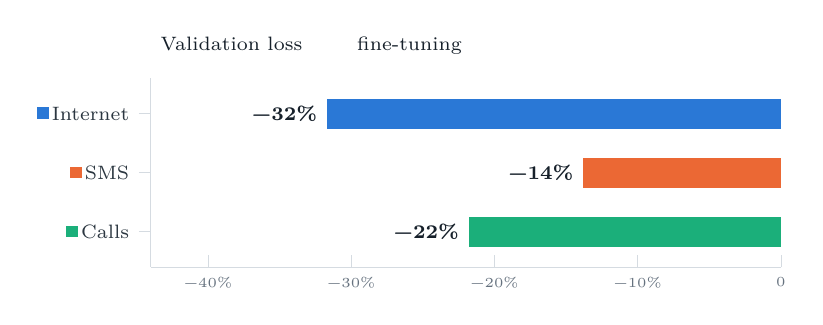
\begin{tikzpicture}
        \begin{axis}[deck, xbar, bar width=0.38cm, bar shift=0pt, width=0.66\linewidth, height=2.4cm, scale only axis,
            xmin=-44, xmax=0, ymin=0.4, ymax=3.6, ytick={1,2,3},
            yticklabels={\sCalls, \sSms, \sInet}, y tick label style={font=\scriptsize, text=text},
            xtick={-40,-30,-20,-10,0}, xticklabels={−40\%, −30\%, −20\%, −10\%, 0},
            nodes near coords, nodes near coords style={font=\scriptsize\bfseries, text=ink, anchor=east},
            point meta=explicit symbolic,
            title={Validation loss μετά το fine-tuning}]
          \addplot[fill=inet, draw=none] coordinates {(-31.7,3) [−32\%]};
          \addplot[fill=sms, draw=none] coordinates {(-13.8,2) [−14\%]};
          \addplot[fill=calls, draw=none] coordinates {(-21.8,1) [−22\%]};
        \end{axis}
      \end{tikzpicture}
      \figcap{Σε σχέση με το zero-shot, στις τελευταίες 5 ημέρες του train.}
    \end{column}
  \end{columns}
\end{frame}
\note{Τα ARIMA και LSTM ξέρουν μόνο ό,τι έμαθαν από τις 6.624 τιμές του train. Το TimesFM ακολουθεί τη λογική των μεγάλων γλωσσικών μοντέλων: η σειρά κόβεται σε κομμάτια των 32 σημείων που παίζουν τον ρόλο των tokens, και η attention συγκρίνει άμεσα το τώρα με την ίδια ώρα πριν από μία εβδομάδα. Στο fine-tuning εκπαιδεύουμε τα δύο τελευταία από τα 20 στρώματα. Όπως και στο LSTM, το validation είναι κανονικές μέρες. Το fine-tuning μειώνει το σφάλμα του validation σε όλες τις σειρές, οπότε εκπρόσωπος της οικογένειας είναι το fine-tuned. Τα βάρη έχουν άδεια μη εμπορικής χρήσης.}

% =====================================================================
\begin{frame}{Ένα μοντέλο αξίζει μόνο αν νικά τον απλό κανόνα}
  \begin{columns}[T, onlytextwidth]
    \begin{column}{0.48\textwidth}
      \begin{block}{Δύο κανόνες που δεν κοστίζουν τίποτα}
        \textbf{Naive}: «η κίνηση θα μείνει όπως είναι».\\
        \textbf{Seasonal naive}: «όπως χθες την ίδια ώρα».
      \end{block}
      \begin{block}{Ένας εκπρόσωπος ανά οικογένεια, επιλεγμένος στο validation}
        ARIMA-x, LSTM μίας ημέρας με από-περιοδικοποίηση, TimesFM fine-tuned.
      \end{block}
    \end{column}
    \begin{column}{0.48\textwidth}
      \small
      \begin{tabular}{@{}>{\raggedright\arraybackslash}p{0.3\textwidth}>{\raggedright\arraybackslash}p{0.64\textwidth}@{}}
        \toprule
        Μετρική & Τι λέει \\
        \midrule
        MAE, RMSE & τυπικό και τετραγωνικό σφάλμα, στις μονάδες της σειράς \\
        MASE & σφάλμα ως κλάσμα του «όπως χθες»· συγκρίνει σειρές \\
        WAPE & ποσοστό του όγκου που προβλέφθηκε λάθος \\
        MAPE & \muted{εκρήγνυται τη νύχτα, όταν η κίνηση πλησιάζει το μηδέν} \\
        \bottomrule
      \end{tabular}
    \end{column}
  \end{columns}
\end{frame}
\note{Όλα τα μοντέλα αξιολογούνται στα ίδια σημεία του test. Μια μετρική μόνη της δεν λέει αν η πρόβλεψη είναι καλή, γι' αυτό συγκρίνουμε με δύο απλούς κανόνες που δεν κοστίζουν τίποτα. Κύρια μετρική είναι η MASE, γιατί δεν εξαρτάται από την κλίμακα. Η MAPE αποτυγχάνει εδώ: στα Calls υπάρχουν 311 δεκάλεπτα με τιμή κάτω από 1, όπου η MAPE φτάνει τις δεκάδες χιλιάδες τοις εκατό. Ένα σφάλμα 2 μονάδων στις 4 το πρωί μετράει όσο εκατοντάδες σφάλματα το μεσημέρι.}

% =====================================================================
\begin{frame}{Το TimesFM έχει το μικρότερο σφάλμα παντού}
  \centering
  \small
  \begin{tabular}{@{}lcccccc@{}}
    \toprule
    & \multicolumn{2}{c}{\sInet} & \multicolumn{2}{c}{\sSms} & \multicolumn{2}{c}{\sCalls} \\
    \cmidrule(lr){2-3}\cmidrule(lr){4-5}\cmidrule(l){6-7}
    MASE & 10\,λεπ. & 50\,λεπ. & 10\,λεπ. & 50\,λεπ. & 10\,λεπ. & 50\,λεπ. \\
    \midrule
    Naive               & 0,302 & 0,480 & 0,602 & 0,759 & 0,438 & 0,599 \\
    ARIMA-x             & 0,296 & 0,433 & 0,580 & 0,724 & 0,410 & 0,520 \\
    LSTM                & 0,409 & 0,592 & 0,646 & 0,791 & 0,496 & 0,578 \\
    TimesFM fine-tuned  & \alert{0,249} & \alert{0,350} & \alert{0,536} & \alert{0,645} & \alert{0,366} & \alert{0,436} \\
    \midrule
    \muted{TimesFM zero-shot} & \muted{0,238} & \muted{0,313} & \muted{0,522} & \muted{0,618} & \muted{0,361} & \muted{0,419} \\
    \bottomrule
  \end{tabular}

  \vspace{0.6em}
  \raggedright\normalsize
  \begin{itemize}
    \item Πρώτο σε κάθε σειρά, ορίζοντα και μετρική (εκτός MAPE). Η zero-shot εκδοχή, \alert{χωρίς καμία εκπαίδευση}, είναι ακόμη λίγο καλύτερη.
    \item Το ARIMA-x είναι λίγο καλύτερο από το Naive. Το LSTM του validation είναι \alert{χειρότερο από το Naive} σε 5 από τις 6 στήλες.
    \item Η δυσκολία είναι ίδια για όλα: Internet < Calls < SMS.
  \end{itemize}
\end{frame}
\note{Στον πίνακα η MASE στο test για τους τρεις εκπροσώπους. Το TimesFM fine-tuned είναι πρώτο σε όλες τις στήλες, και η zero-shot εκδοχή, στην τελευταία γραμμή, είναι ακόμη καλύτερη: το fine-tuning βοήθησε στο validation αλλά όχι στο test. Το LSTM εδώ είναι 9 έως 38\% χειρότερο από το ARIMA-x, το αντίθετο από το 84 έως 87\% υπέρ του LSTM στο άρθρο των Siami-Namini: οι σειρές μας είναι κυρίως γραμμικές και περιοδικές, ενώ οι οικονομικές σειρές του άρθρου έχουν τάσεις, και το test μας έχει γιορτές. Η seasonal naive, όπως χθες, είναι παντού τελευταία, γιατί αποτυγχάνει στις γιορτές και στη μετάβαση προς το Σαββατοκύριακο.}

% =====================================================================
\begin{frame}{Μόνο το TimesFM νικά καθαρά τον απλό κανόνα}
  \centering
  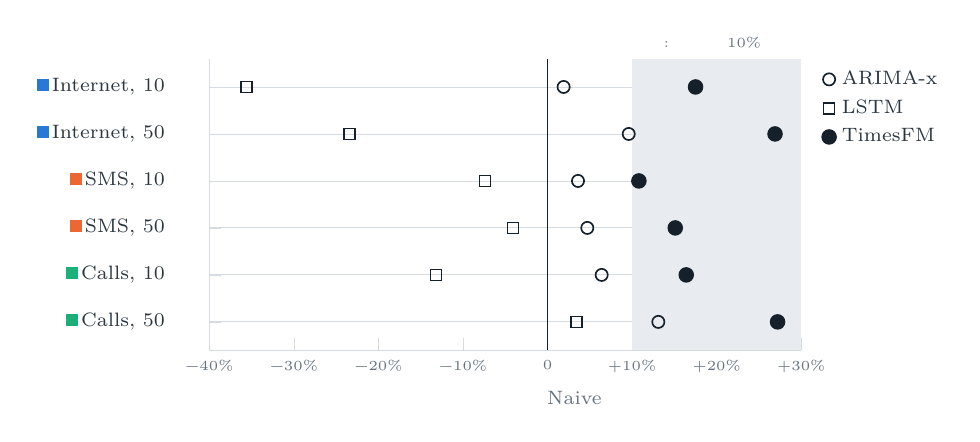
\begin{tikzpicture}
    \begin{axis}[deck, width=0.62\textwidth, height=3.7cm, scale only axis,
        xmin=-40, xmax=30, ymin=0.4, ymax=6.6,
        xtick={-40,-30,-20,-10,0,10,20,30}, xticklabels={−40\%, −30\%, −20\%, −10\%, 0, +10\%, +20\%, +30\%},
        ytick={1,...,6}, y tick label style={font=\scriptsize, text=text},
        yticklabels={{\ser{calls}{Calls}, 50 λεπτά}, {\ser{calls}{Calls}, 10 λεπτά},
                     {\ser{sms}{SMS}, 50 λεπτά}, {\ser{sms}{SMS}, 10 λεπτά},
                     {\ser{inet}{Internet}, 50 λεπτά}, {\ser{inet}{Internet}, 10 λεπτά}},
        xlabel={μικρότερο σφάλμα από το Naive},
        ymajorgrids, major grid style={draw=rule, line width=0.3pt},
        legend style={at={(1.02,1)}, anchor=north west}, legend cell align=left, clip=false]
      \fill[fillc] (axis cs:10,0.4) rectangle (axis cs:30,6.6);
      \node[anchor=south west, font=\tiny, text=muted, inner xsep=0pt] at (axis cs:10,6.62) {επιτυχία: τουλάχιστον 10\%};
      \draw[ink, line width=0.5pt] (axis cs:0,0.4) -- (axis cs:0,6.6);
      \addplot[only marks, mark=o, mark size=2.2pt, draw=ink, line width=0.6pt]
        coordinates {(1.9,6) (9.6,5) (3.6,4) (4.7,3) (6.4,2) (13.1,1)};
      \addlegendentry{ARIMA-x}
      \addplot[only marks, mark=square, mark size=2pt, draw=ink, line width=0.6pt]
        coordinates {(-35.6,6) (-23.4,5) (-7.4,4) (-4.1,3) (-13.2,2) (3.4,1)};
      \addlegendentry{LSTM}
      \addplot[only marks, mark=*, mark size=2.6pt, fill=ink, draw=ink]
        coordinates {(17.5,6) (26.9,5) (10.8,4) (15.1,3) (16.4,2) (27.2,1)};
      \addlegendentry{TimesFM}
    \end{axis}
  \end{tikzpicture}

  \vspace{0.4em}
  \raggedright
  Το Naive δεν κοστίζει τίποτα, άρα είναι το \alert{πραγματικό κατώφλι}. Το ARIMA-x το περνά σε όλες τις περιπτώσεις αλλά οριακά, το LSTM σχεδόν πουθενά.
\end{frame}
\note{Η MASE κάτω από 1 είναι πολύ χαλαρό κριτήριο: το περνά ακόμη και το Naive. Το πραγματικό κατώφλι είναι η βελτίωση έναντι του Naive. Ορίσαμε επιτυχία ως τουλάχιστον 10\% μικρότερο σφάλμα· το όριο είναι δική μας επιλογή, και φαίνεται ως η σκιασμένη ζώνη. Το TimesFM, οι γεμάτοι κύκλοι, είναι μέσα στη ζώνη σε κάθε γραμμή, με 11 έως 27\%. Το ARIMA-x είναι πάντα πάνω από το μηδέν αλλά μπαίνει στη ζώνη μόνο στα Calls για 50 λεπτά. Το LSTM που διάλεξε το validation είναι κάτω από το Naive παντού εκτός από τα Calls για 50 λεπτά, κυρίως λόγω των γιορτών, όπως θα δούμε.}

% =====================================================================
\begin{frame}{Όλα πιάνουν το σχήμα, κανένα την αιχμή της Πρωτοχρονιάς}
  \begin{columns}[T, onlytextwidth]
    \begin{column}{0.64\textwidth}
      \IfFileExists{figs/forecast_holidays.dat}{%
        \begin{tikzpicture}
          \begin{groupplot}[deck, group style={group size=1 by 2, vertical sep=0.45cm, xticklabels at=edge bottom},
              width=0.9\linewidth, height=1.9cm, scale only axis, xmin=0, xmax=9, ymin=0,
              xtick={0,...,8}, xticklabels={24/12,25/12,26/12,27/12,28/12,29/12,30/12,31/12,1/1},
              legend style={at={(0,-0.38)}, anchor=north west, legend columns=4}, unbounded coords=jump]
            \nextgroupplot[ymax=2100, title={\sInet}]
              \addplot[quiet, line width=0.4pt, dotted] table[x=x, y=inet_arima] {figs/forecast_holidays.dat};
              \addplot[quiet, line width=0.4pt, dashed] table[x=x, y=inet_lstm] {figs/forecast_holidays.dat};
              \addplot[ink, line width=0.5pt] table[x=x, y=inet_tfm] {figs/forecast_holidays.dat};
              \addplot[inet, line width=1pt, opacity=0.85] table[x=x, y=inet_actual] {figs/forecast_holidays.dat};
            \nextgroupplot[ymax=1650, title={\sSms}]
              \addplot[quiet, line width=0.4pt, dotted] table[x=x, y=sms_arima] {figs/forecast_holidays.dat};
              \addlegendentry{ARIMA}
              \addplot[quiet, line width=0.4pt, dashed] table[x=x, y=sms_lstm] {figs/forecast_holidays.dat};
              \addlegendentry{LSTM}
              \addplot[ink, line width=0.5pt] table[x=x, y=sms_tfm] {figs/forecast_holidays.dat};
              \addlegendentry{TimesFM}
              \addplot[sms, line width=1pt, opacity=0.85] table[x=x, y=sms_actual] {figs/forecast_holidays.dat};
              \addlegendentry{πραγματική τιμή}
          \end{groupplot}
        \end{tikzpicture}
        \figcap{24/12 έως 01/01, πρόβλεψη 50 λεπτών.}%
      }{%
        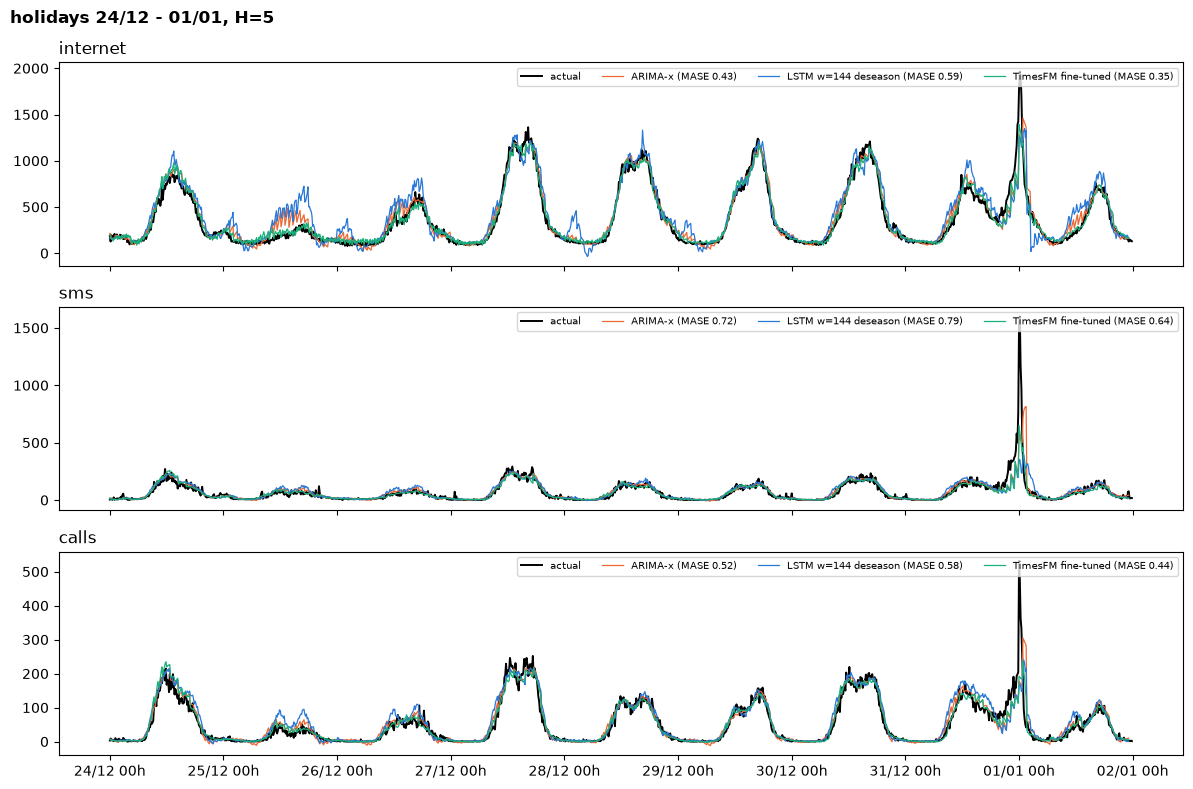
\includegraphics[width=\linewidth, height=0.66\textheight, keepaspectratio]{forecast_holidays.png}
        \figcap{24/12 έως 01/01, πρόβλεψη 50 λεπτών. Μαύρο: πραγματική τιμή. Πορτοκαλί: ARIMA-x, μπλε: LSTM, πράσινο: TimesFM.}%
      }
    \end{column}
    \begin{column}{0.33\textwidth}
      \small
      \begin{itemize}
        \item Το ημερήσιο σχήμα το πιάνουν \alert{όλα}.
        \item 25–26/12: τα μοντέλα του train, κυρίως το LSTM, περιμένουν κανονική μέρα και \alert{υπερεκτιμούν}. Το TimesFM προσαρμόζεται πιο γρήγορα.
        \item Την αιχμή της Πρωτοχρονιάς \alert{δεν την προβλέπει κανείς}· εμφανίζεται στην πρόβλεψη με καθυστέρηση.
      \end{itemize}
    \end{column}
  \end{columns}
\end{frame}
\note{Στις κανονικές μέρες οι προβλέψεις σχεδόν καλύπτουν την πραγματική σειρά, και οι διαφορές αφορούν το ύψος της κορυφής. Τα μεγάλα σφάλματα είναι στις ώρες κίνησης, όπου ένα λάθος προκαλεί συμφόρηση. Στις γιορτές τα μοντέλα του train υπερεκτιμούν. Την αιχμή της Πρωτοχρονιάς, περίπου 70 φορές τα κανονικά SMS σε 10 λεπτά, δεν την προβλέπει κανένα μοντέλο από το ιστορικό· για τέτοια γεγονότα χρειάζεται ημερολόγιο εκδηλώσεων.}

% =====================================================================
\begin{frame}{Ό,τι βοήθησε στο validation, έβλαψε στις γιορτές}
  \begin{columns}[T, onlytextwidth]
    \begin{column}{0.6\textwidth}
      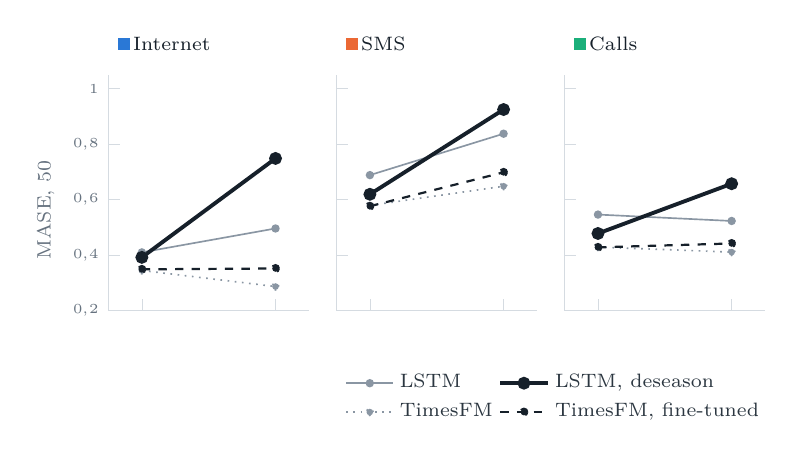
\begin{tikzpicture}
        \begin{groupplot}[deck, group style={group size=3 by 1, horizontal sep=0.35cm, yticklabels at=edge left},
            width=0.21\textwidth, height=3.0cm, scale only axis, xmin=-0.25, xmax=1.25, ymin=0.2, ymax=1.05,
            xtick={0,1}, xticklabels={κανονικές, γιορτές}, ytick={0.2,0.4,0.6,0.8,1},
            yticklabel style={/pgf/number format/use comma, /pgf/number format/fixed},
            legend style={at={(0,-0.22)}, anchor=north west, legend columns=2}, legend cell align=left]
          \nextgroupplot[title={\sInet}, ylabel={MASE, 50 λεπτά}]
            \addplot[quiet, line width=0.6pt, mark=*, mark size=1.2pt] coordinates {(0,0.410) (1,0.496)};
            \addplot[ink, line width=1.4pt, mark=*, mark size=1.6pt] coordinates {(0,0.392) (1,0.748)};
            \addplot[quiet, line width=0.6pt, dotted, mark=*, mark size=1.2pt] coordinates {(0,0.345) (1,0.287)};
            \addplot[ink, line width=0.8pt, dashed, mark=*, mark size=1.2pt] coordinates {(0,0.349) (1,0.352)};
          \nextgroupplot[title={\sSms}]
            \addplot[quiet, line width=0.6pt, mark=*, mark size=1.2pt] coordinates {(0,0.688) (1,0.837)};
            \addlegendentry{LSTM}
            \addplot[ink, line width=1.4pt, mark=*, mark size=1.6pt] coordinates {(0,0.619) (1,0.924)};
            \addlegendentry{LSTM, deseason}
            \addplot[quiet, line width=0.6pt, dotted, mark=*, mark size=1.2pt] coordinates {(0,0.579) (1,0.648)};
            \addlegendentry{TimesFM}
            \addplot[ink, line width=0.8pt, dashed, mark=*, mark size=1.2pt] coordinates {(0,0.576) (1,0.698)};
            \addlegendentry{TimesFM, fine-tuned}
          \nextgroupplot[title={\sCalls}]
            \addplot[quiet, line width=0.6pt, mark=*, mark size=1.2pt] coordinates {(0,0.546) (1,0.523)};
            \addplot[ink, line width=1.4pt, mark=*, mark size=1.6pt] coordinates {(0,0.478) (1,0.657)};
            \addplot[quiet, line width=0.6pt, dotted, mark=*, mark size=1.2pt] coordinates {(0,0.429) (1,0.411)};
            \addplot[ink, line width=0.8pt, dashed, mark=*, mark size=1.2pt] coordinates {(0,0.428) (1,0.442)};
        \end{groupplot}
      \end{tikzpicture}
      \figcap{Κανονικές: 17–23/12. Γιορτές: 24/12–01/01. Μικρότερο είναι καλύτερο.}
    \end{column}
    \begin{column}{0.37\textwidth}
      \small
      \begin{itemize}
        \item Η από-περιοδικοποίηση βοηθά στις κανονικές μέρες, αλλά στις γιορτές το σφάλμα ανεβαίνει \alert{40–90\%}.
        \item Το fine-tuning δεν αλλάζει τις κανονικές μέρες και \alert{χειροτερεύει τις γιορτές}.
        \item Ταιριάζει καλύτερα στο παρελθόν $\neq$ προβλέπει καλύτερα ένα μέλλον που αλλάζει.
      \end{itemize}
    \end{column}
  \end{columns}
\end{frame}
\note{Χωρίζουμε το test σε κανονικές μέρες και γιορτές. Οι σκούρες γραμμές είναι τα δύο κόλπα που βελτίωσαν το validation: η από-περιοδικοποίηση, η παχιά γραμμή, ανεβαίνει απότομα στις γιορτές σε κάθε σειρά. Στο test η τυπική απόκλιση του υπολοίπου είναι 2,3 έως 3,5 φορές μεγαλύτερη από το train, οπότε ένα μοντέλο που περιμένει κανονική μέρα κάνει μεγάλα λάθη. Το απλό LSTM και το TimesFM zero-shot ακολουθούν το πρόσφατο επίπεδο και αντέχουν καλύτερα. Και οι δύο σκούρες γραμμές είναι οι εκπρόσωποι που διάλεξε το validation: το test δείχνει το κόστος αυτής της επιλογής, που δεν μπορούσαμε να το δούμε από πριν.}

% =====================================================================
\begin{frame}{Τα διαστήματα του TimesFM ακολουθούν την ώρα}
  \begin{columns}[T, onlytextwidth]
    \begin{column}{0.5\textwidth}
      \small
      \begin{tabular}{@{}lccc@{}}
        \toprule
        95\%, 10 λεπτά & \sInet & \sSms & \sCalls \\
        \midrule
        \multicolumn{4}{@{}l}{\muted{κάλυψη (στόχος 95\%)}} \\
        ARIMA-x & 98\% & 92\% & 93\% \\
        TimesFM & 93\% & 91\% & 95\% \\
        \midrule
        \multicolumn{4}{@{}l}{\muted{πλάτος, σχετικά}} \\
        ARIMA-x & 2,08 & 2,91 & 2,29 \\
        TimesFM & \alert{1,20} & \alert{2,19} & \alert{1,79} \\
        \bottomrule
      \end{tabular}
      \figcap{TimesFM fine-tuned. Πλάτος ως πολλαπλάσιο της κλίμακας της MASE.}
    \end{column}
    \begin{column}{0.47\textwidth}
      \begin{itemize}
        \item Το ARIMA-x έχει \alert{σταθερό πλάτος}: πολύ φαρδύ τη νύχτα, πολύ στενό στην αιχμή.
        \item Το TimesFM \alert{προσαρμόζεται}: 22–42\% στενότερο, με κάλυψη 91–95\%.
        \item Τα σημεία εκτός είναι κυρίως από πάνω: τις ανοδικές αιχμές δεν τις προβλέπει κανείς.
      \end{itemize}
    \end{column}
  \end{columns}
\end{frame}
\note{Για τη διαστασιολόγηση χρειαζόμαστε ένα εύρος, όχι μόνο μια τιμή. Το ARIMA δίνει διάστημα με σταθερό πλάτος, που τη νύχτα πηγαίνει και κάτω από το μηδέν. Το TimesFM δίνει ποσοστημόρια, οπότε το διάστημα αλλάζει με την ώρα. Τα σημεία εκτός είναι κυρίως από πάνω, γιατί τις ανοδικές αιχμές δεν τις προβλέπει κανείς. Η υποκάλυψη θα μπορούσε να διορθωθεί με conformal prediction. Τηλεπικοινωνιακά μετράει το άνω όριο: αν δεσμεύουμε χωρητικότητα ίση με αυτό, η ζήτηση την ξεπερνά περίπου στο 2,5\% των δεκαλέπτων.}

% =====================================================================
\begin{frame}{Σφάλμα 6–9\% του όγκου χωράει στο περιθώριο χωρητικότητας}
  \begin{columns}[T, onlytextwidth]
    \begin{column}{0.48\textwidth}
      \begin{itemize}
        \item \textbf{Internet}: το TimesFM κάνει λάθος στο \alert{6–9\%} του όγκου, κάτω από το συνηθισμένο περιθώριο (15–30\%). Τα carriers ανοίγουν πριν την αιχμή.
        \item \textbf{Νύχτα}: χαμηλή κίνηση, μικρό σφάλμα. Ο εξοπλισμός κλείνει με ασφάλεια.
        \item \textbf{Νέες κυψέλες}: το καλύτερο μοντέλο στο test, το TimesFM zero-shot, \alert{δεν χρειάζεται εκπαίδευση ανά κυψέλη}.
      \end{itemize}
    \end{column}
    \begin{column}{0.48\textwidth}
      \small
      \begin{tabular}{@{}lll@{}}
        \toprule
        & Εκπαίδευση & Ανά πρόβλεψη \\
        \midrule
        ARIMA-x & \textasciitilde 11 s ανά fit & \textasciitilde 1,4 s με νέο fit \\
        LSTM & 4–17 λεπτά & < 1 ms \\
        TimesFM & 0 ή \textasciitilde 27 λεπτά & \textasciitilde 48 ms, batch \\
        \bottomrule
      \end{tabular}
      \figcap{CPU χωρίς GPU. Για 10.000 κυψέλες το TimesFM θέλει \textasciitilde 8 λεπτά ανά κύκλο των 10 λεπτών, το ARIMA-x με νέο fit σε κάθε βήμα \textasciitilde 4 ώρες.}
    \end{column}
  \end{columns}
\end{frame}
\note{Με σφάλμα 6 έως 9\% του όγκου στο Internet, ο πάροχος ξέρει 10 έως 50 λεπτά πριν πόση χωρητικότητα θα χρειαστεί. Τη νύχτα μπορεί να κλείσει εξοπλισμό για εξοικονόμηση ενέργειας. Η υποεκτίμηση κοστίζει περισσότερο από την υπερεκτίμηση, οπότε η διαστασιολόγηση πρέπει να γίνεται με ένα άνω όριο της πρόβλεψης. Αιχμές και γιορτές θέλουν ημερολόγιο εκδηλώσεων και περιθώριο ασφαλείας. Στην πράξη θα προτείναμε το TimesFM σε GPU στον Non-RT RIC για προβλέψεις λεπτών, και ελαφριά μοντέλα στον Near-RT RIC για γρήγορες διορθώσεις και ως εφεδρικά.}

% =====================================================================
\begin{frame}{Συμπεράσματα}
  \begin{enumerate}
    \item Στα 10 λεπτά η τελευταία τιμή είναι ήδη καλή πρόβλεψη. Ένα μοντέλο αξίζει μόνο αν \alert{νικά το Naive}.
    \vspace{0.5em}
    \item Το ARIMA-x νικά το Naive οριακά. Το LSTM του validation δεν το νικά σχεδόν πουθενά.
    \vspace{0.5em}
    \item Το \alert{TimesFM} κερδίζει παντού, κατά 11–27\% έναντι του Naive, και δίνει καλύτερα διαστήματα. Χωρίς fine-tuning κερδίζει ακόμη περισσότερο (13–35\%).
    \vspace{0.5em}
    \item Ό,τι βελτίωσε το validation δεν βοήθησε στις γιορτές: \alert{το μέλλον δεν μοιάζει πάντα με το παρελθόν}.
    \vspace{0.5em}
    \item Αιχμές όπως της Πρωτοχρονιάς δεν προβλέπονται από το ιστορικό μόνο.
  \end{enumerate}
\end{frame}
\note{Κλείνοντας: η persistence είναι ισχυρό σημείο αναφοράς στα 10 λεπτά. Το TimesFM κερδίζει παντού, και μάλιστα καλύτερα χωρίς εκπαίδευση, αλλά κοστίζει περισσότερο στο inference. Και η επιλογή με βάση το validation μπορεί να παραπλανήσει όταν το test περιέχει συνθήκες που δεν έχουμε δει. Ευχαριστούμε.}

\end{document}
